\exer{Parcours en largeur -- Applications}
\begin{flushright}
\textit{D'après ressources Jules Svartz, Lycée Masséna.}
\end{flushright}

Soit le graphe ci-dessous. 

\begin{center}
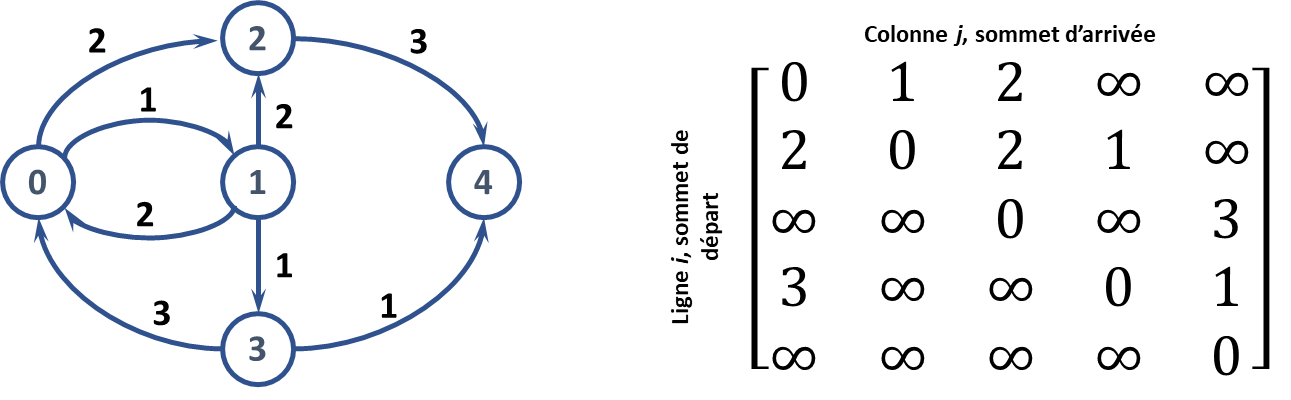
\includegraphics[width=7cm]{graphe_01}
\end{center}

\question{Modéliser le graphe ci-dessus en utilisant un dictionnaire d'adjacence nommé \texttt{G1}. On rappelle que dans ce cas, les clés seront des chaînes de caractère désignant le numéro du sommet et les valeurs seront constituées de la liste de chaînes de caractères où ces chaînes désignent les sommets successeurs.}


\question{Ecrire la procédure \texttt{parcours\_largeur(g,s) -> None} réalisant le parcours en largeur d'un graphe, à partir du sommet \texttt{s}.}
%\begin{lstlisting}
%
%\end{lstlisting}

On souhaite disposer de la fontion  \texttt{parcours\_largeur\_distances(g,s) -> dict}. Cette fonction renverra le disctionnaire contenant toutes les distances à \texttt{s} en nombre de sommets. On va pour cela modifier la procédure précédente ainsi :
\begin{itemize}
\item  les sommets visités seront stockés dans un dictionnaire \texttt{distances} où les clés seront les \texttt{n} sommets du graphe. Chacune des valeurs sera initialisée à l'infini (\texttt{float('inf')}), sauf la valeur associée au sommet de départ qui sera \texttt{0};
\item à chaque fois que le voisin \texttt{v} d'un sommet \texttt{u} est ajouté à la file d'attente des sommets à traiter, 
si \texttt{distances[v]=inf} alors \texttt{distances[v]} prendra la valeur 1+\texttt{distances[u]} .
\end{itemize}

\question{Implémenter  la fontion  \texttt{parcours\_largeur\_distances(g,s) -> dict}. Dans le second exemple, comment interpréter les \texttt{inf} ?}
\begin{exemple}~\\
\vspace{-.5cm}
\begin{lstlisting}
>>> parcours_largeur_distances(G1,"0")
	{'0': 0, '1': 1, '2': 2, '3': 3, '4': 1, '5': 2, '6': 2, '7': 3}
>>> parcours_largeur_distances(G1,"2")
	{'0': inf, '1': inf, '2': 0, '3': 1, '4': inf, '5': inf, '6': 1, '7': 2}
\end{lstlisting}
\end{exemple}
On souhaite maintenant connaître la liste des prédécesseurs de chaque sommet dans le cadre d'un parcours en largeur. On dit que $u$ est le prédécesseur de $v$ dans la parcours en largeur si $v$ est découvert pour la première fois dans la liste d'adjacence de $u$. Dans ce cas, on a donc \texttt{distances[v]=distances[u]+1}.  On pourra initialiser un dictionnaire  \texttt{predecesseurs} de taille \texttt{n} ayant uniquement des \texttt{-1} comme valeur. À la fin du parcours on aura \texttt{predecesseurs[v]=-1} si \texttt{v} est le sommet de départ ou si \texttt{v} n'est pas accessible depuis le sommet de départ. 

\question{Implémenter  la fontion  \texttt{parcours\_largeur\_predecesseurs(graphe,s) -> dict} renvoyant le dictionnaire des prédécesseurs du sommet \texttt{s}.}
\begin{exemple}~\\
\vspace{-.5cm}
\begin{lstlisting}
>>> parcours_largeur_predecesseurs(G1,"0")
	{'0': -1, '1': '0', '2': '1', '3': '2', '4': '0', '5': '1', '6': '1', '7': '6'}
>>> parcours_largeur_predecesseurs(G1,"2")
	{'0': -1, '1': -1, '2': -1, '3': '2', '4': -1, '5': -1, '6': '2', '7': '3'}
\end{lstlisting}
\end{exemple}
%\begin{lstlisting}
%>>> parcours_largeur(G1, 0)
%([0, 1, 2, 3, 1, 2, 2, 3], [-1, 0, 1, 2, 0, 4, 1, 6])
%>>> parcours_largeur(G1, 2)
%([inf, inf, 0, 1, inf, inf, 1, 2], [-1, -1, -1, 2, -1, -1, 2, 6])
%\end{lstlisting}

 À partir de la liste \texttt{predecesseurs} précédente, il est possible de calculer
effectivement des plus courts chemins : pour calculer le plus court chemin de \texttt{s} à \texttt{v} (avec \texttt{v} accessible depuis \texttt{s}), il
suffit de remonter de prédecesseur en prédecesseur de \texttt{v} jusqu’à \texttt{s} grâce à la liste \texttt{predecesseurs} : on obtient alors le chemin à
l’envers.

\question{Écrire une fonction \texttt{chemin(g,s,v)} prenant en entrée un graphe, les sommets \texttt{s} de départ et \texttt{v} d'arrivée, et renvoyant, dans l’ordre, un plus court chemin de \texttt{s} à \texttt{v}. La fonction renverra une liste vide si le chemin n'existe pas.}

\begin{exemple}~\\
\vspace{-.5cm}
\begin{lstlisting}
>>> chemin(G1,"0","6")
	['0', '1', '6']
>>> chemin(G1,"2","1")
	[]
\end{lstlisting}
\end{exemple}

%\begin{lstlisting}
%>>> chemin(parcours_largeur(G1,0)[1], 0, 7)
%[0, 1, 6, 7]
%\end{lstlisting}